\documentclass[letterpaper, 12pt]{article}

\usepackage{hyperref}
\usepackage{pgfplots}
\usepgfplotslibrary{fillbetween}


\title{Basics of Economics}
\author{Alvin Lin}
\date{Principles of Microeconomics: August 2016 - December 2016}

\begin{document}

\maketitle

\section{Governments and Markets}

\subsection{Price Ceilings}
A \textbf{price ceiling} is a regulation making it illegal to charge more than
specified price. A price ceiling set above the equilibrium price has no effect.
A price ceiling set below the equilibrium price results in dead-weight loss.

\subsubsection{Consequences of a Binding Price Ceiling}
\begin{itemize}
  \item Shortage
  \item A transfer of surplus from producers to consumers
  \item Deadweight loss
  \item Producer surplus decreases
  \item Consumer surplus increases
\end{itemize}

\subsubsection{Rent Ceilings}
A \textbf{rent ceiling} is a government regulation making it illegal to charge
a rent higher than a specified level. Landlords will restrict the supply in
response while the quantity demanded increases. This causes a housing shortage,
dead-weight loss, and a transfer of surplus from landlords to renters. The
opportunity costs to renters increases since finding an apartment requires more
search.

\subsubsection{Consequences of Rent Ceilings}
The rent ceiling encourages an illegal market for apartments. Renters and
landlords figure out ways to increase the rents. Landlords introduce
``additional service'' charges and engage in side deals. The effects of black
market activities is determined by how strictly enforced rent control is.
If the control is lax, the black market price is very close to the market price.
If the control is strict, the black market price is much higher than the market
price.

\subsubsection{Example}
\begin{center}
  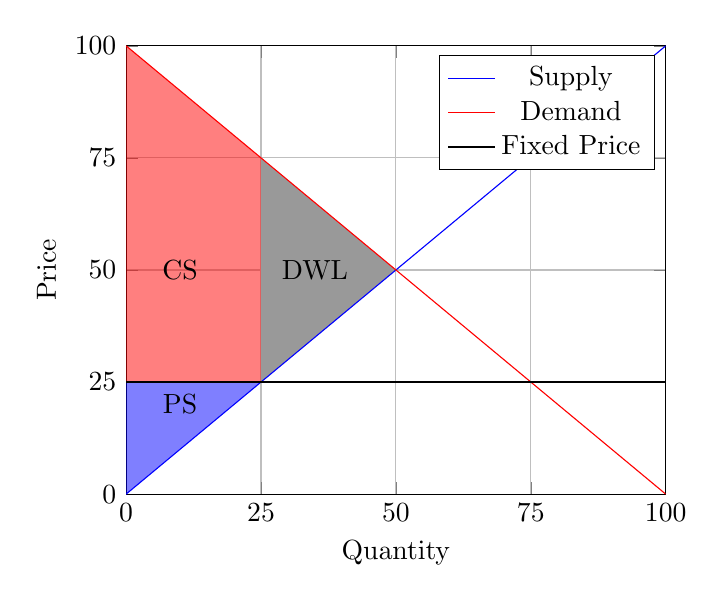
\begin{tikzpicture}
    \begin{axis} [
      xlabel={Quantity}, ylabel={Price},
      xtick={0,25,50,75,100}, ytick={0,25,50,75,100},
      xmin=0, xmax=100, ymin=0, ymax=100,
      grid=both
    ]
      \addplot[name path=supply, color=blue] coordinates { (0,0) (100,100) };
      \addlegendentry{Supply};
      \addplot[name path=demand, color=red] coordinates { (0,100) (100,0) };
      \addlegendentry{Demand};
      \addplot[name path=split, color=black] coordinates { (0,25) (100,25) };
      \addlegendentry{Fixed Price};
      \addplot[color=blue, fill=blue, fill opacity=0.5]
        fill between [of=split and supply, soft clip={domain=0:25}];
      \addplot[color=red, fill=red, fill opacity=0.5]
        fill between [of=split and demand, soft clip={domain=0:25}];
      \addplot[color=black, fill=black!40]
        fill between [of=supply and demand, soft clip={domain=25:50}];
      \node[draw=none] at (10,50) {CS};
      \node[draw=none] at (10,20) {PS};
      \node[draw=none] at (35,50) {DWL};
    \end{axis}
  \end{tikzpicture}
\end{center}
At the equilibrium price, there was no dead-weight loss, with the consumer
and producer surplus equal to 1250. At a fixed price of 25, there is align
dead-weight loss of 625. The new consumer surplus is 1562.5. The new
producer surplus is 312.5. The total surplus is 1875.
\[ \Delta CS = +312.5 \]
\[ \Delta PS = -937.5 \]
\[ \Delta TS = -625 \]

\subsection{Price Floors}
A \textbf{price floor} is a regulation making it illegal to charge less than a
specified price. A price floor set below the equilibrium price has no effect.
A price floor set above the equilibrium price results in dead-weight loss.

\subsubsection{Consequences of a Binding Price Floor}
\begin{itemize}
  \item Surplus
  \item A transfer of surplus from consumers to producers
  \item Deadweight loss
  \item Consumer surplus decreases
  \item Producer surplus increases
\end{itemize}

\subsubsection{Minimum Wage}
\textbf{Minimum wage} is a government regulation making it illegal to pay a
worker less than a specified wage. It is a price floor imposed on the labor
market. The labor market has a supply of labor (workers), and demand for labor
(producers of goods and services).

\subsubsection{Consequences of a Minimum Wage}
\begin{itemize}
  \item Unemployment
  \item Deadweight loss
  \item A transfer of surplus from employees to workers
  \item Consumer surplus decreases
  \item Producer surplus increases or decreases
  \item Benefits workers that keep their jobs
  \item Hurts people that are looking for work and those that lose their jobs
\end{itemize}

\subsubsection{Example}
\[ Supply: P = 1+Q \]
\[ Demand: P = 16-2Q \]
\[ S = D \]
\[ 1+Q^{*} = 16-2Q^{*} \]
\[ 3Q^{*} = 15 \]
\[ Q^{*} = 5 \]
\begin{center}
  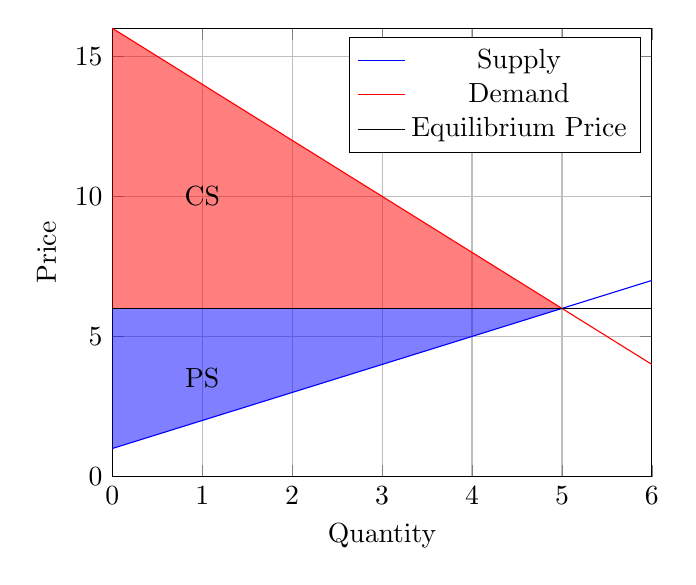
\begin{tikzpicture}
    \begin{axis} [
      xlabel={Quantity}, ylabel={Price},
      xmin=0, xmax=6, ymin=0, ymax=16,
      grid=both
    ]
      \addplot[name path=supply, color=blue] coordinates { (0,1) (6,7) };
      \addlegendentry{Supply};
      \addplot[name path=demand, color=red] coordinates { (0,16) (6,4) };
      \addlegendentry{Demand};
      \addplot[name path=split, color=black] coordinates { (0,6) (6,6) };
      \addlegendentry{Equilibrium Price};
      \addplot[color=blue, fill=blue, fill opacity=0.5]
        fill between [of=split and supply, soft clip={domain=0:5}];
      \addplot[color=red, fill=red, fill opacity=0.5]
        fill between [of=split and demand, soft clip={domain=0:5}];
      \node[draw=none] at (1,10) {CS};
      \node[draw=none] at (1,3.5) {PS};
    \end{axis}
  \end{tikzpicture}
\end{center}
At \( Q^{*} \):
\[ PS = \frac{1}{2}bh = \frac{1}{2}(5)(5) = 12.5 \]
\[ CS = \frac{1}{2}bh = \frac{1}{2}(10)(5) = 25 \]
\[ TS = 37.5 \]
What is the effect of a minimum wage of \$10 on consumer surplus, producer
surplus, and total surplus?
\begin{center}
  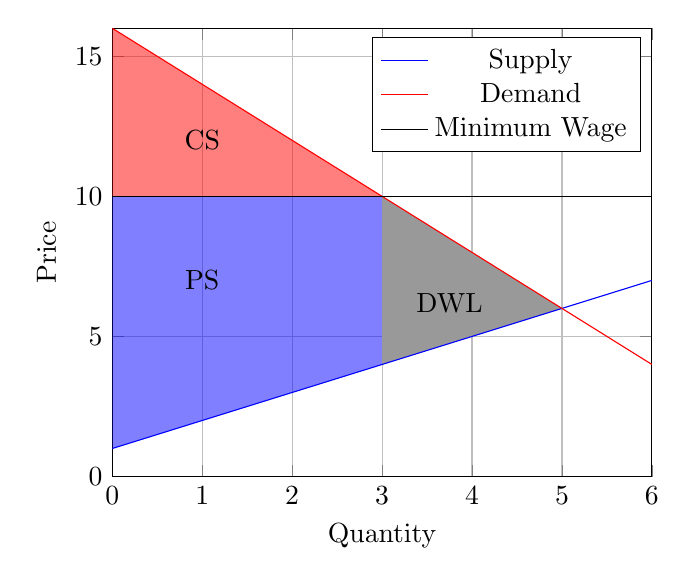
\begin{tikzpicture}
    \begin{axis} [
      xlabel={Quantity}, ylabel={Price},
      xmin=0, xmax=6, ymin=0, ymax=16,
      grid=both
    ]
      \addplot[name path=supply, color=blue] coordinates { (0,1) (6,7) };
      \addlegendentry{Supply};
      \addplot[name path=demand, color=red] coordinates { (0,16) (6,4) };
      \addlegendentry{Demand};
      \addplot[name path=split, color=black] coordinates { (0,10) (6,10) };
      \addlegendentry{Minimum Wage};
      \addplot[color=blue, fill=blue, fill opacity=0.5]
        fill between [of=split and supply, soft clip={domain=0:3}];
      \addplot[color=red, fill=red, fill opacity=0.5]
        fill between [of=split and demand, soft clip={domain=0:3}];
      \addplot[color=black, fill=black!40]
        fill between [of=supply and demand, soft clip={domain=3:5}];
      \node[draw=none] at (1,12) {CS};
      \node[draw=none] at (1,7) {PS};
      \node[draw=none] at (3.75,6.2) {DWL};
    \end{axis}
  \end{tikzpicture}
\end{center}
At the fixed minimum wage:
\[ PS = \frac{1}{2}(b_{1}+b_{2})h = \frac{1}{2}(9+6)(3) = 22.5 \]
\[ CS = \frac{1}{2}bh = \frac{1}{2}(3)(6) = 9 \]
\[ TS = 31.5 \]
Change:
\[ \Delta PS = 10 \]
\[ \Delta CS = -16 \]
\[ \Delta TS = -6 \]

\subsection{Taxes}
A tax a levy imposed on an individual or other legal entity by the state.
Failure to pay is punishable by law. In the market, a tax on sellers is a fixed
fee per unit sold. A tax on buyers is a fixed fee for each unit purchased. \par
Other taxes include taxes on trade, proportional taxes on expenditure or
revenue, estate taxes, gift taxes, and fixed flat taxes.

\subsubsection{Key Questions}
\begin{itemize}
  \item How much tax revenue is raised?
  \item Does the tax result in an inefficient quantity traded?
  \item Who bears the burden of the tax?
  \item What are the effects on producer surplus, consumer surplus, and total
  surplus.
\end{itemize}

\subsubsection{Tax Incidence}
\textbf{Tax Incidence} is the division of the burden of a tax between buyers
and sellers. If a tax is imposed on the sale of a good, the price faced by
consumers might increase by the whole amount, part of it, or by nothing at all.
If the price does not change, then the cost of the tax is borne by sellers. \par
It does not matter whether the consumer or the producer is taxed.

\subsubsection{Consequences of Taxes}
\begin{itemize}
  \item Increases in the price
  \item Decrease in quantity traded
  \item Producer surplus and consumer surplus decrease
  \item Deadweight loss
  \item Tax revenue raised by the government
\end{itemize}

\subsubsection{Example}
Suppose the government imposes a \$2 tax on sellers:
\begin{center}
  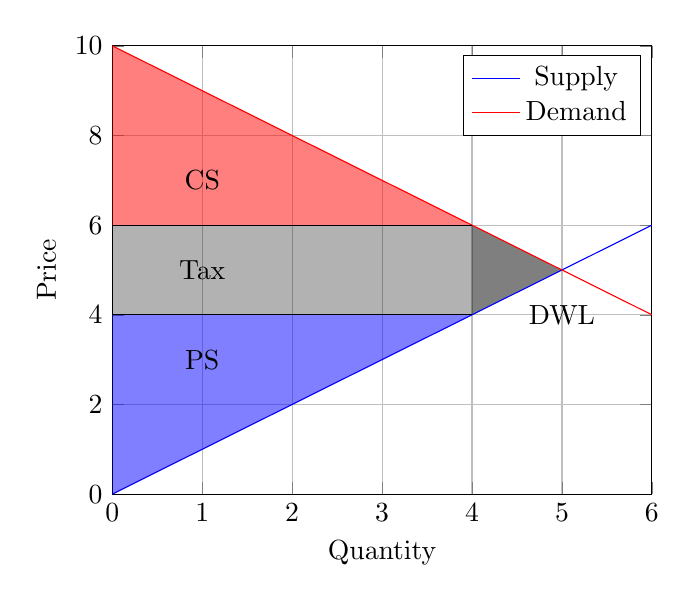
\begin{tikzpicture}
    \begin{axis} [
      xlabel={Quantity}, ylabel={Price},
      xmin=0, xmax=6, ymin=0, ymax=10,
      grid=both
    ]
      \addplot[name path=supply, color=blue] coordinates { (0,0) (6,6) };
      \addlegendentry{Supply};
      \addplot[name path=demand, color=red] coordinates { (0,10) (6,4) };
      \addlegendentry{Demand};
      \addplot[name path=tax1, color=black] coordinates { (0,4) (4,4) };
      \addplot[name path=tax2, color=black] coordinates { (0,6) (4,6) };
      \addplot[color=blue, fill=blue, fill opacity=0.5]
        fill between [of=tax1 and supply, soft clip={domain=0:4}];
      \addplot[color=red, fill=red, fill opacity=0.5]
        fill between [of=tax2 and demand, soft clip={domain=0:4}];
      \addplot[color=black, fill=black, fill opacity=0.3]
        fill between [of=tax1 and tax2, soft clip={domain=0:4}];
      \addplot[color=black, fill=black, fill opacity=0.5]
        fill between [of=supply and demand, soft clip={domain=4:5}];
      \node[draw=none] at (1,7) {CS};
      \node[draw=none] at (1,3) {PS};
      \node[draw=none] at (1,5) {Tax};
      \node[draw=none] at (5,4) {DWL};
    \end{axis}
  \end{tikzpicture}
\end{center}

\subsubsection{Practice Problem}
Brownies:
\begin{center}
  \begin{tabular}{|c|c|c|}
    \hline
    P       & \( Q_{D} \) & \( Q_{S} \) \\ \hline
    \$0.50  & 5           & 3           \\ \hline
    \$0.60  & 4           & 4           \\ \hline
    \$0.70  & 3           & 5           \\ \hline
    \$0.80  & 2           & 6           \\ \hline
    \$0.90  & 1           & 7           \\ \hline
  \end{tabular}
\end{center}
What is \( Q_{*} \) and \( P_{*} \) with no tax?
\[ P_{*} = 0.60 \quad Q_{*} = 4 \]
If sellers are taxed \$0.10 per brownie and buyers taxed \$0.10 per brownie,
then the price paid is \$0.70 per brownie and the price received is \$0.50 per
brownie. The quantity demanded and supplied is 3.

\subsection{Subsidies}
A subsidy is a payment made by the government to a producer, or a consumer.
A subsidy has the opposite effect of a tax.

\subsubsection{Example}
Suppose there is a \$20 subsidy to sellers:
\begin{center}
  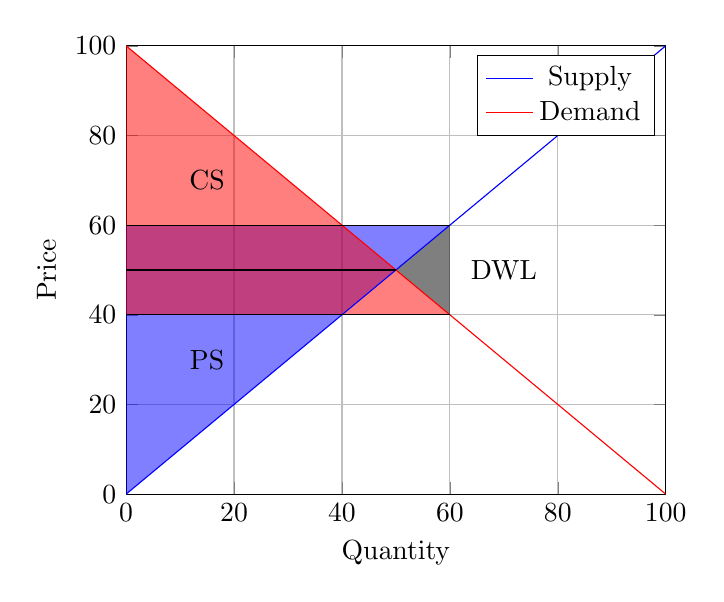
\begin{tikzpicture}
    \begin{axis} [
      xlabel={Quantity}, ylabel={Price},
      xmin=0, xmax=100, ymin=0, ymax=100,
      grid=both
    ]
      \addplot[name path=supply, color=blue] coordinates { (0,0) (100,100) };
      \addlegendentry{Supply};
      \addplot[name path=demand, color=red] coordinates { (0,100) (100,0) };
      \addlegendentry{Demand};
      \addplot[name path=subsidy1, color=black] coordinates { (0,60) (60,60) };
      \addplot[name path=subsidy2, color=black] coordinates { (0,40) (60,40) };
      \addplot[name path=split, color=black] coordinates { (0,50) (50,50) };
      \addplot[color=blue, fill=blue, fill opacity=0.5]
        fill between [of=subsidy1 and supply, soft clip={domain=0:60}];
      \addplot[color=red, fill=red, fill opacity=0.5]
        fill between [of=subsidy2 and demand, soft clip={domain=0:60}];
      \addplot[color=black, fill=black, fill opacity=0.5]
        fill between [of=supply and demand, soft clip={domain=50:60}];
      \node[draw=none] at (15,70) {CS};
      \node[draw=none] at (15,30) {PS};
      \node[draw=none] at (70,50) {DWL};
    \end{axis}
  \end{tikzpicture}
\end{center}
The consumer surplus and producer surplus both increase by 550. The cost of the
policy is 1200 (the rectangular region including the surpluses and the
dead-weight loss), so the total surplus decreases. \par
If a \$10 tax is imposed on buyers and a \$10 subsidy is imposed on sellers,
both curve shifts cancel and there is no net effect.

\subsubsection{Consequences of Subsidies}
\begin{itemize}
  \item Increases in supply
  \item Decrease in price
  \item Inefficient overproduction
  \item Consumer surplus and producer surplus increase
  \item Increases in surplus are offset by the cost of the subsidy, resulting in
  deadweight loss
\end{itemize}

\subsection{Production Quotas}
A production quota is an upper limit on the amount of a good that can be
produced. It is usually intended to help producers by raising prices.

\subsubsection{Consequences of a Production Quota}
\begin{itemize}
  \item Increase in price
  \item Decrease in consumer surplus
  \item Increase in producer surplus
  \item Transfer of surplus from consumers to producers
  \item Deadweight loss
  \item Provides an incentive for producers to cheat and overproduce
\end{itemize}

\subsection{Markets for Illegal Goods}
If illegal goods are taxed, it raises tax revenue for the government. On the
other hand, the government profits from the trade of harmful substances.
Formerly illegal drugs are now legitimate and thus might influence the
preferences of consumers.

\begin{center}
  You can find all my notes at \url{http://omgimanerd.tech/notes}. If you have
  any questions, comments, or concerns, please contact me at
  alvin@omgimanerd.tech
\end{center}

\end{document}
